\chapter{Аралық сұратымдар}

\index{аралық сұратымдар}
\index{қосынды сұратымы}
\index{минимум сұратымы}
\index{максимум сұратымы}

Бұл тарауда аралық сұратымдарды тиімді өңдейтін
деректер құрылымдары жайлы сөз қозғайтын боламыз.
Әдетте \key{аралық сұратымдар} есепте
ішжиымдарға негізделген мәндерді табуға арналады.
Қарапайым аралық сұратымдар:
\begin{itemize}
\item $\texttt{sum}_q(a,b)$: $[a,b]$ аралығындағы сандардың қосындысын есептеу
\item $\texttt{min}_q(a,b)$: $[a,b]$ аралығындағы сандардың минимумын есептеу
\item $\texttt{max}_q(a,b)$: $[a,b]$ аралығындағы сандардың максимумын есептеу
\end{itemize}

Мысалы, төмендегі жиымдағы $[3,6]$ арасын қарастырайық:
\begin{center}
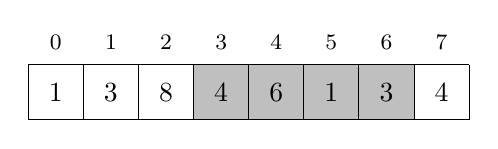
\begin{tikzpicture}[scale=0.7]
\fill[color=lightgray] (3,0) rectangle (7,1);
\draw (0,0) grid (8,1);

\node at (0.5,0.5) {$1$};
\node at (1.5,0.5) {$3$};
\node at (2.5,0.5) {$8$};
\node at (3.5,0.5) {$4$};
\node at (4.5,0.5) {$6$};
\node at (5.5,0.5) {$1$};
\node at (6.5,0.5) {$3$};
\node at (7.5,0.5) {$4$};

\footnotesize
\node at (0.5,1.4) {$0$};
\node at (1.5,1.4) {$1$};
\node at (2.5,1.4) {$2$};
\node at (3.5,1.4) {$3$};
\node at (4.5,1.4) {$4$};
\node at (5.5,1.4) {$5$};
\node at (6.5,1.4) {$6$};
\node at (7.5,1.4) {$7$};
\end{tikzpicture}
\end{center}
Қарастырылған жағдайда $\texttt{sum}_q(3,6)=14$,
$\texttt{min}_q(3,6)=1$ және $\texttt{max}_q(3,6)=6$.

Бұл аралық сұратымды өңдеудің ең қарапайым жолы --
аралықтың барлық элементтерін өтіп шығатын циклды қолдану.
Мысалы, төмендегі функция қосынды сұратымдарын өңдейді:

\begin{lstlisting}
int sum(int a, int b) {
    int s = 0;
    for (int i = a; i <= b; i++) {
        s += array[i];
    }
    return s;
}
\end{lstlisting}

Функция $O(n)$ уақытта жұмыс жасайды,
мұндағы $n$ -- жиымның өлшемі. Демек $q$ сұратымды
$O(nq)$ уақытта өңдейміз. Егер 
$n$ мен $q$ екеуі де үлкен болса, бұл 
тәсіл біз үшін баяу. Бақытымызға орай, аралық сұратымдарды
әлдеқайда тезірек өңдеу жолдары да бар. 

\section{Статикалық жиым сұратымдары}

Алдымен жиым \emph{статикалық} болатын (яғни жиымның 
мәндері сұратым араларында өзгермейтін) жағдайды
қарастырайық. Бұл жағдайда барлық сұратымдарға жауап беретін 
статикалық деректер құрылымын құрыстыру жеткілікті.

\subsubsection{Қосынды сұратымдары}

\index{префиксті қосындылар жиымы}

\key{Префиксті қосындылар жиымын} құрыстыру арқылы
біз статикалық жиымның 
қосынды сұратымдарын жеңіл есептей аламыз.
Префиксті қосындылар жиымындағы әр мән 
негізгі жиымдағы алғашқы элементтен бастап сол позицияға дейінгі сандардың қосындысына тең болады,
яғни $k$ позициясындағы мән $\texttt{sum}_q(0,k)$-ға тең. 
Префиксті қосындылар жиымы $O(n)$ уақытта құрастырылады.

Мысалы төмендегі жиымды қарастырайық:
\begin{center}
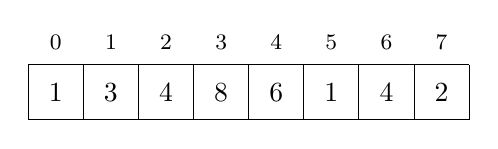
\begin{tikzpicture}[scale=0.7]
%\fill[color=lightgray] (3,0) rectangle (7,1);
\draw (0,0) grid (8,1);

\node at (0.5,0.5) {$1$};
\node at (1.5,0.5) {$3$};
\node at (2.5,0.5) {$4$};
\node at (3.5,0.5) {$8$};
\node at (4.5,0.5) {$6$};
\node at (5.5,0.5) {$1$};
\node at (6.5,0.5) {$4$};
\node at (7.5,0.5) {$2$};

\footnotesize
\node at (0.5,1.4) {$0$};
\node at (1.5,1.4) {$1$};
\node at (2.5,1.4) {$2$};
\node at (3.5,1.4) {$3$};
\node at (4.5,1.4) {$4$};
\node at (5.5,1.4) {$5$};
\node at (6.5,1.4) {$6$};
\node at (7.5,1.4) {$7$};
\end{tikzpicture}
\end{center}
Оған сәйкес префиксті қосындылар жиымы:
\begin{center}
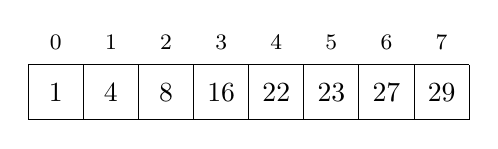
\begin{tikzpicture}[scale=0.7]
%\fill[color=lightgray] (3,0) rectangle (7,1);
\draw (0,0) grid (8,1);

\node at (0.5,0.5) {$1$};
\node at (1.5,0.5) {$4$};
\node at (2.5,0.5) {$8$};
\node at (3.5,0.5) {$16$};
\node at (4.5,0.5) {$22$};
\node at (5.5,0.5) {$23$};
\node at (6.5,0.5) {$27$};
\node at (7.5,0.5) {$29$};


\footnotesize
\node at (0.5,1.4) {$0$};
\node at (1.5,1.4) {$1$};
\node at (2.5,1.4) {$2$};
\node at (3.5,1.4) {$3$};
\node at (4.5,1.4) {$4$};
\node at (5.5,1.4) {$5$};
\node at (6.5,1.4) {$6$};
\node at (7.5,1.4) {$7$};
\end{tikzpicture}
\end{center}
Жиым $\texttt{sum}_q(0,k)$-ның 
барлық мәндерін қамтығандықтан,
біз қалаған $\texttt{sum}_q(a,b)$ мәнін $O(1)$ 
уақытта төмендегідей жолмен таба аламыз:
\[ \texttt{sum}_q(a,b) = \texttt{sum}_q(0,b) - \texttt{sum}_q(0,a-1)\]
$\texttt{sum}_q(0,-1)=0$ деп санасақ, 
$a=0$ болған жағдайда да формула жұмыс жасай береді. 

Мысалы, $[3,6]$ аралығын қарастырайық:
\begin{center}
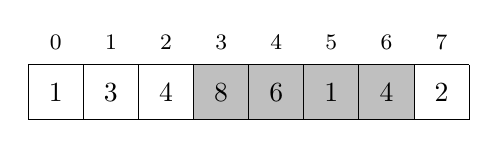
\begin{tikzpicture}[scale=0.7]
\fill[color=lightgray] (3,0) rectangle (7,1);
\draw (0,0) grid (8,1);

\node at (0.5,0.5) {$1$};
\node at (1.5,0.5) {$3$};
\node at (2.5,0.5) {$4$};
\node at (3.5,0.5) {$8$};
\node at (4.5,0.5) {$6$};
\node at (5.5,0.5) {$1$};
\node at (6.5,0.5) {$4$};
\node at (7.5,0.5) {$2$};

\footnotesize
\node at (0.5,1.4) {$0$};
\node at (1.5,1.4) {$1$};
\node at (2.5,1.4) {$2$};
\node at (3.5,1.4) {$3$};
\node at (4.5,1.4) {$4$};
\node at (5.5,1.4) {$5$};
\node at (6.5,1.4) {$6$};
\node at (7.5,1.4) {$7$};
\end{tikzpicture}
\end{center}
Бұл жағдайда $\texttt{sum}_q(3,6)=8+6+1+4=19$.
Қосындыны префиксті қосыныдылар жиымының екі мәні
арқылы есептей аламыз:
\begin{center}
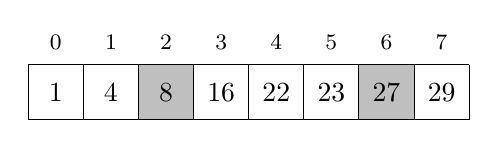
\begin{tikzpicture}[scale=0.7]
\fill[color=lightgray] (2,0) rectangle (3,1);
\fill[color=lightgray] (6,0) rectangle (7,1);
\draw (0,0) grid (8,1);

\node at (0.5,0.5) {$1$};
\node at (1.5,0.5) {$4$};
\node at (2.5,0.5) {$8$};
\node at (3.5,0.5) {$16$};
\node at (4.5,0.5) {$22$};
\node at (5.5,0.5) {$23$};
\node at (6.5,0.5) {$27$};
\node at (7.5,0.5) {$29$};

\footnotesize
\node at (0.5,1.4) {$0$};
\node at (1.5,1.4) {$1$};
\node at (2.5,1.4) {$2$};
\node at (3.5,1.4) {$3$};
\node at (4.5,1.4) {$4$};
\node at (5.5,1.4) {$5$};
\node at (6.5,1.4) {$6$};
\node at (7.5,1.4) {$7$};
\end{tikzpicture}
\end{center}
Осылайша $\texttt{sum}_q(3,6)=\texttt{sum}_q(0,6)-\texttt{sum}_q(0,2)=27-8=19$.

Бұл идеяны әрі қарай көп өлшемдерге 
жалпылауға болады. Мысалы, екі өлшемді 
префиксті қосындылар жиымын құрастырып, 
төртбұрыш ішжиымдардың қосындыларын $O(1)$ 
уақытта таба аламыз. Жиымдағы әр қосынды
жоғарғы сол жақ бұрыштан басталатын ішжиымға
есептеледі. 

\begin{samepage}
Төмендегі сурет аталған идеяны бейнелейді:
\begin{center}
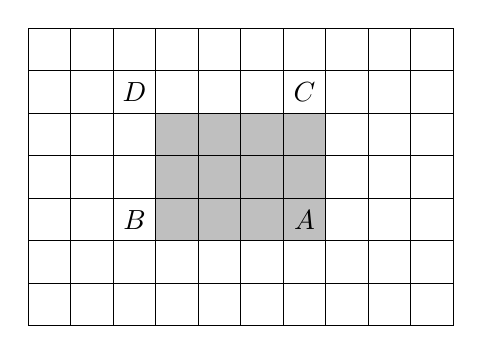
\begin{tikzpicture}[scale=0.54]
\draw[fill=lightgray] (3,2) rectangle (7,5);
\draw (0,0) grid (10,7);
\node[anchor=center] at (6.5, 2.5) {$A$};
\node[anchor=center] at (2.5, 2.5) {$B$};
\node[anchor=center] at (6.5, 5.5) {$C$};
\node[anchor=center] at (2.5, 5.5) {$D$};
\end{tikzpicture}
\end{center}
\end{samepage}

Сұр түспен белгіленіп тұрған ішжиымның қосындысын
\[S(A) - S(B) - S(C) + S(D)\]
формуласы арқылы табуға болады,
мұндағы $S(X)$ үстіңгі сол жақ бұрыштан басталып,
$X$ позициясында аяқталатын ішжиым мәндерінің қосындысы. 

\subsubsection{Минимум сұратымдары}

\index{сиретілген кесте}

Минимум сұратымдарын өңдеу қосынды сұратымдарды 
өңдеуден қиынырақ. Дегенмен $O(n \log n)$ уақыт ішінде
алдын ала өңдеу арқылы кез келген минимум сұратымдарын $O(1)$
уақытта таба аламыз\footnote{Бұл техника алғаш 
\cite{ben00} көрсетілді және кейде 
\key{сиретілген кесте} әдісі деп аталады.
Күрделі техникалар \cite{fis06} арқылы алдын 
ала өңдеу уақыты $O(n)$ болатын алгоритмдер де бар, бірақ олар
спорттық бағдарламалауда қажетсіз.}.
Максимум мен минимум сұратымдары бірдей өңделетіндіктен,
минимум сұратымдарын ғана қарастырайық.

Идеясы барлық $\textrm{min}_q(a,b)$ мәндерін 
алдын ала есептеуге негізделеді. Мұндағы $b-a+1$ (аралықтың ұзындығы) 
екінің дәрежесі. 
Мысалы, төмендегі жиым үшін

\begin{center}
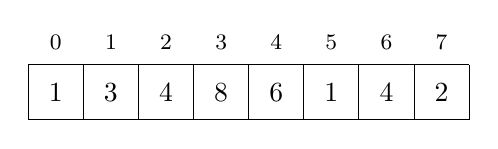
\begin{tikzpicture}[scale=0.7]
\draw (0,0) grid (8,1);

\node at (0.5,0.5) {$1$};
\node at (1.5,0.5) {$3$};
\node at (2.5,0.5) {$4$};
\node at (3.5,0.5) {$8$};
\node at (4.5,0.5) {$6$};
\node at (5.5,0.5) {$1$};
\node at (6.5,0.5) {$4$};
\node at (7.5,0.5) {$2$};

\footnotesize
\node at (0.5,1.4) {$0$};
\node at (1.5,1.4) {$1$};
\node at (2.5,1.4) {$2$};
\node at (3.5,1.4) {$3$};
\node at (4.5,1.4) {$4$};
\node at (5.5,1.4) {$5$};
\node at (6.5,1.4) {$6$};
\node at (7.5,1.4) {$7$};
\end{tikzpicture}
\end{center}
келесі мәндер есептеледі:

\begin{center}
\begin{tabular}{ccc}

\begin{tabular}{lll}
$a$ & $b$ & $\texttt{min}_q(a,b)$ \\
\hline
0 & 0 & 1 \\
1 & 1 & 3 \\
2 & 2 & 4 \\
3 & 3 & 8 \\
4 & 4 & 6 \\
5 & 5 & 1 \\
6 & 6 & 4 \\
7 & 7 & 2 \\
\end{tabular}

&

\begin{tabular}{lll}
$a$ & $b$ & $\texttt{min}_q(a,b)$ \\
\hline
0 & 1 & 1 \\
1 & 2 & 3 \\
2 & 3 & 4 \\
3 & 4 & 6 \\
4 & 5 & 1 \\
5 & 6 & 1 \\
6 & 7 & 2 \\
\\
\end{tabular}

&

\begin{tabular}{lll}
$a$ & $b$ & $\texttt{min}_q(a,b)$ \\
\hline
0 & 3 & 1 \\
1 & 4 & 3 \\
2 & 5 & 1 \\
3 & 6 & 1 \\
4 & 7 & 1 \\
0 & 7 & 1 \\
\\
\\
\end{tabular}

\end{tabular}
\end{center}

Алдын ала есептелген мәндердің саны $O(n \log n)$,
себебі ұзындығы екінің дәрежесі болатын аралықтардың саны $O(\log n)$.
Мәндер келесі рекурсиялық формула арқылы тиімді 
есептеледі:
\[\texttt{min}_q(a,b) = \min(\texttt{min}_q(a,a+w-1),\texttt{min}_q(a+w,b)),\]
мұндағы $b-a+1$ екінің дәрежесі және $w=(b-a+1)/2$.
Барлық мәндерді есептеу $O(n \log n)$ уақыт алады.

Осыдан кейін кез келген $\texttt{min}_q(a,b)$ мәнін
екі алдын ала есептелген мән арқылы $O(1)$ уақытта 
есептей аламыз. $k$ деп $b-a+1$-ден аспайтын 
екінің ең үлкен дәрежесін алайық.
$\texttt{min}_q(a,b)$ мәнін төмендегі формула арқылы есептеуге болады:
\[\texttt{min}_q(a,b) = \min(\texttt{min}_q(a,a+k-1),\texttt{min}_q(b-k+1,b)).\]
Формулада $[a,b]$ аралығы ұзындықтары $k$ болатын 
$[a,a+k-1]$ және $[b-k+1,b]$ аралықтарының бірігуі деп көрсетілген.


Мысалы, $[1,6]$ аралығын қарастырайық:
\begin{center}
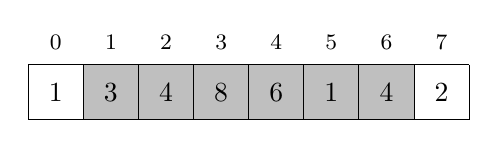
\begin{tikzpicture}[scale=0.7]
\fill[color=lightgray] (1,0) rectangle (7,1);
\draw (0,0) grid (8,1);

\node at (0.5,0.5) {$1$};
\node at (1.5,0.5) {$3$};
\node at (2.5,0.5) {$4$};
\node at (3.5,0.5) {$8$};
\node at (4.5,0.5) {$6$};
\node at (5.5,0.5) {$1$};
\node at (6.5,0.5) {$4$};
\node at (7.5,0.5) {$2$};

\footnotesize
\node at (0.5,1.4) {$0$};
\node at (1.5,1.4) {$1$};
\node at (2.5,1.4) {$2$};
\node at (3.5,1.4) {$3$};
\node at (4.5,1.4) {$4$};
\node at (5.5,1.4) {$5$};
\node at (6.5,1.4) {$6$};
\node at (7.5,1.4) {$7$};
\end{tikzpicture}
\end{center}
Аралықтың ұзындығы -- 6, ал
6-дан аспайтын екінің ең үлкен дәрежесі -- 4.
Ендеше, $[1,6]$ аралығы -- $[1,4]$ аралығы мен
$[3,6]$ аралығының бірігуінен тұрады.
\begin{center}
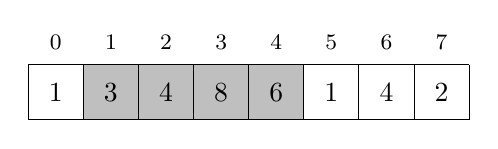
\begin{tikzpicture}[scale=0.7]
\fill[color=lightgray] (1,0) rectangle (5,1);
\draw (0,0) grid (8,1);

\node at (0.5,0.5) {$1$};
\node at (1.5,0.5) {$3$};
\node at (2.5,0.5) {$4$};
\node at (3.5,0.5) {$8$};
\node at (4.5,0.5) {$6$};
\node at (5.5,0.5) {$1$};
\node at (6.5,0.5) {$4$};
\node at (7.5,0.5) {$2$};

\footnotesize
\node at (0.5,1.4) {$0$};
\node at (1.5,1.4) {$1$};
\node at (2.5,1.4) {$2$};
\node at (3.5,1.4) {$3$};
\node at (4.5,1.4) {$4$};
\node at (5.5,1.4) {$5$};
\node at (6.5,1.4) {$6$};
\node at (7.5,1.4) {$7$};
\end{tikzpicture}
\end{center}
\begin{center}
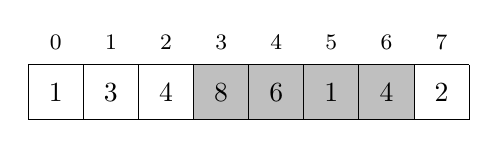
\begin{tikzpicture}[scale=0.7]
\fill[color=lightgray] (3,0) rectangle (7,1);
\draw (0,0) grid (8,1);

\node at (0.5,0.5) {$1$};
\node at (1.5,0.5) {$3$};
\node at (2.5,0.5) {$4$};
\node at (3.5,0.5) {$8$};
\node at (4.5,0.5) {$6$};
\node at (5.5,0.5) {$1$};
\node at (6.5,0.5) {$4$};
\node at (7.5,0.5) {$2$};


\footnotesize
\node at (0.5,1.4) {$0$};
\node at (1.5,1.4) {$1$};
\node at (2.5,1.4) {$2$};
\node at (3.5,1.4) {$3$};
\node at (4.5,1.4) {$4$};
\node at (5.5,1.4) {$5$};
\node at (6.5,1.4) {$6$};
\node at (7.5,1.4) {$7$};
\end{tikzpicture}
\end{center}
$\texttt{min}_q(1,4)=3$ және $\texttt{min}_q(3,6)=1$ болғандықтан,
$\texttt{min}_q(1,6)=1$ деп тұжырымдаймыз.

\section{Бинарлы индекстелген дарақ}

\index{бинарлы индекстелген дарақ}
\index{Фенвик дарағы}

\key{Бинарлы индекстелген дарақ} немесе \key{Фенвик дарағын}
\footnote{Бинарлы индекстелген дарақты 1994 жылы П.М.Фенвик ұсынды \cite{fen94}.} префиксті қосындының динамикалық нұсқасы деп
қарастыруға болады. Ол жиымға қатысты екі операцияны -- аралық 
қосындыны табу мен мәнді өзгертуді $O(\log n)$ уақытта орындайды.

Бинарлы индекстелген дарақтың артықшылығы -- 
аралық қосындылармен қатар жиымдағы мәндерді тиімді өзгертуінде.
Бұл қасиет префиксті қосындылар жиымында жоқ.  
Әр жаңарту операциясы префиксті қосындылар жиымын басынан бастап
қайта құрастыратындықтан, ол $O(n)$ уақыт алады. 

\subsubsection{Құрылымы}

Құрылымның аты бинарлы индекстелген \emph{дарақ} болғанымен, 
әдетте ол жиым ретінде көрсетіледі. Бұл бөлімде жиымды
бірлік индекстелген деп қарастырамыз, себебі ол кодтың жазылу барысын
жеңілдетеді. 

$p(k)$ деп $k$-ні бөле алатын ең үлкен екінің дәрежесін
белгілейік. Бинарлы индекстелген дарақты 
\[ \texttt{tree}[k] = \texttt{sum}_q(k-p(k)+1,k)\]
болатындай \texttt{tree} жиымында сақтаймыз,
яғни әр $k$ позициясында берілген жиымның ұзындығы
$p(k)$ болатын және $k$ позициясында бітетін аралықтың
қосындысын сақтаймыз. 
Мысалы, $p(6)=2$ болғандықтан $\texttt{tree}[6]$
$\texttt{sum}_q(5,6)$ мәнін сақтайды. 

Өрнек ретінде төмендегі жиымды қарастырайық:
\begin{center}
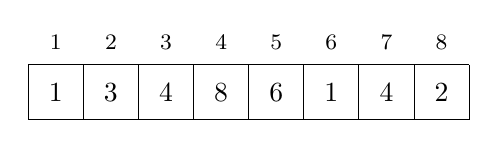
\begin{tikzpicture}[scale=0.7]
\draw (0,0) grid (8,1);

\node at (0.5,0.5) {$1$};
\node at (1.5,0.5) {$3$};
\node at (2.5,0.5) {$4$};
\node at (3.5,0.5) {$8$};
\node at (4.5,0.5) {$6$};
\node at (5.5,0.5) {$1$};
\node at (6.5,0.5) {$4$};
\node at (7.5,0.5) {$2$};

\footnotesize
\node at (0.5,1.4) {$1$};
\node at (1.5,1.4) {$2$};
\node at (2.5,1.4) {$3$};
\node at (3.5,1.4) {$4$};
\node at (4.5,1.4) {$5$};
\node at (5.5,1.4) {$6$};
\node at (6.5,1.4) {$7$};
\node at (7.5,1.4) {$8$};
\end{tikzpicture}
\end{center}

Осыған сәйкес бинарлы индекстелген дарақ:
\begin{center}
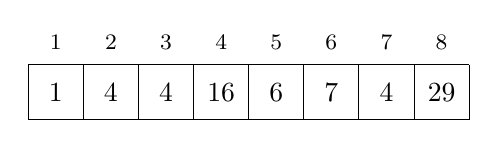
\begin{tikzpicture}[scale=0.7]
\draw (0,0) grid (8,1);

\node at (0.5,0.5) {$1$};
\node at (1.5,0.5) {$4$};
\node at (2.5,0.5) {$4$};
\node at (3.5,0.5) {$16$};
\node at (4.5,0.5) {$6$};
\node at (5.5,0.5) {$7$};
\node at (6.5,0.5) {$4$};
\node at (7.5,0.5) {$29$};

\footnotesize
\node at (0.5,1.4) {$1$};
\node at (1.5,1.4) {$2$};
\node at (2.5,1.4) {$3$};
\node at (3.5,1.4) {$4$};
\node at (4.5,1.4) {$5$};
\node at (5.5,1.4) {$6$};
\node at (6.5,1.4) {$7$};
\node at (7.5,1.4) {$8$};
\end{tikzpicture}
\end{center}

Төмендегі сурет бинарлы индекстелген дарақтың
әр мәнінің әуелгі жиымдағы қандай аралыққа 
сәйкестігін анық көрсетеді:

\begin{center}
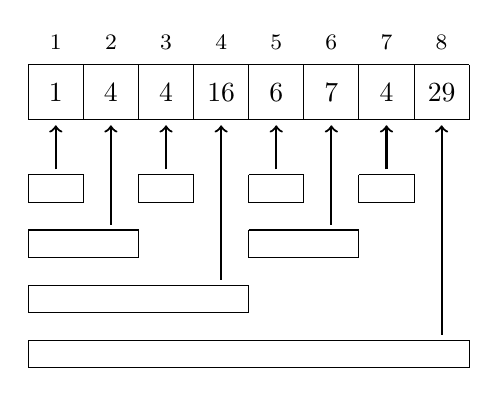
\begin{tikzpicture}[scale=0.7]
\draw (0,0) grid (8,1);

\node at (0.5,0.5) {$1$};
\node at (1.5,0.5) {$4$};
\node at (2.5,0.5) {$4$};
\node at (3.5,0.5) {$16$};
\node at (4.5,0.5) {$6$};
\node at (5.5,0.5) {$7$};
\node at (6.5,0.5) {$4$};
\node at (7.5,0.5) {$29$};

\footnotesize
\node at (0.5,1.4) {$1$};
\node at (1.5,1.4) {$2$};
\node at (2.5,1.4) {$3$};
\node at (3.5,1.4) {$4$};
\node at (4.5,1.4) {$5$};
\node at (5.5,1.4) {$6$};
\node at (6.5,1.4) {$7$};
\node at (7.5,1.4) {$8$};

\draw[->,thick] (0.5,-0.9) -- (0.5,-0.1);
\draw[->,thick] (2.5,-0.9) -- (2.5,-0.1);
\draw[->,thick] (4.5,-0.9) -- (4.5,-0.1);
\draw[->,thick] (6.5,-0.9) -- (6.5,-0.1);
\draw[->,thick] (1.5,-1.9) -- (1.5,-0.1);
\draw[->,thick] (5.5,-1.9) -- (5.5,-0.1);
\draw[->,thick] (3.5,-2.9) -- (3.5,-0.1);
\draw[->,thick] (7.5,-3.9) -- (7.5,-0.1);

\draw (0,-1) -- (1,-1) -- (1,-1.5) -- (0,-1.5) -- (0,-1);
\draw (2,-1) -- (3,-1) -- (3,-1.5) -- (2,-1.5) -- (2,-1);
\draw (4,-1) -- (5,-1) -- (5,-1.5) -- (4,-1.5) -- (4,-1);
\draw (6,-1) -- (7,-1) -- (7,-1.5) -- (6,-1.5) -- (6,-1);
\draw (0,-2) -- (2,-2) -- (2,-2.5) -- (0,-2.5) -- (0,-2);
\draw (4,-2) -- (6,-2) -- (6,-2.5) -- (4,-2.5) -- (4,-2);
\draw (0,-3) -- (4,-3) -- (4,-3.5) -- (0,-3.5) -- (0,-3);
\draw (0,-4) -- (8,-4) -- (8,-4.5) -- (0,-4.5) -- (0,-4);
\end{tikzpicture}
\end{center}

Қарастырылған дарақ арқылы
қалаған $\texttt{sum}_q(1,k)$ мәнін 
$O(\log n)$ уақытта есептей аламыз.
Себебі $[1,k]$ аралығын әрдайым 
қосындылары дарақта сақталатын $O(\log n)$ аралыққа бөлуге болады. 

Мысалы, $[1,7]$ аралығы төмендегідей аралықтарға 
бөлінеді:
\begin{center}
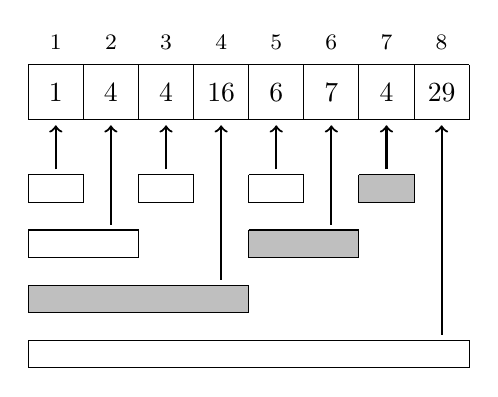
\begin{tikzpicture}[scale=0.7]
\draw (0,0) grid (8,1);

\node at (0.5,0.5) {$1$};
\node at (1.5,0.5) {$4$};
\node at (2.5,0.5) {$4$};
\node at (3.5,0.5) {$16$};
\node at (4.5,0.5) {$6$};
\node at (5.5,0.5) {$7$};
\node at (6.5,0.5) {$4$};
\node at (7.5,0.5) {$29$};

\footnotesize
\node at (0.5,1.4) {$1$};
\node at (1.5,1.4) {$2$};
\node at (2.5,1.4) {$3$};
\node at (3.5,1.4) {$4$};
\node at (4.5,1.4) {$5$};
\node at (5.5,1.4) {$6$};
\node at (6.5,1.4) {$7$};
\node at (7.5,1.4) {$8$};

\draw[->,thick] (0.5,-0.9) -- (0.5,-0.1);
\draw[->,thick] (2.5,-0.9) -- (2.5,-0.1);
\draw[->,thick] (4.5,-0.9) -- (4.5,-0.1);
\draw[->,thick] (6.5,-0.9) -- (6.5,-0.1);
\draw[->,thick] (1.5,-1.9) -- (1.5,-0.1);
\draw[->,thick] (5.5,-1.9) -- (5.5,-0.1);
\draw[->,thick] (3.5,-2.9) -- (3.5,-0.1);
\draw[->,thick] (7.5,-3.9) -- (7.5,-0.1);

\draw (0,-1) -- (1,-1) -- (1,-1.5) -- (0,-1.5) -- (0,-1);
\draw (2,-1) -- (3,-1) -- (3,-1.5) -- (2,-1.5) -- (2,-1);
\draw (4,-1) -- (5,-1) -- (5,-1.5) -- (4,-1.5) -- (4,-1);
\draw[fill=lightgray] (6,-1) -- (7,-1) -- (7,-1.5) -- (6,-1.5) -- (6,-1);
\draw (0,-2) -- (2,-2) -- (2,-2.5) -- (0,-2.5) -- (0,-2);
\draw[fill=lightgray] (4,-2) -- (6,-2) -- (6,-2.5) -- (4,-2.5) -- (4,-2);
\draw[fill=lightgray] (0,-3) -- (4,-3) -- (4,-3.5) -- (0,-3.5) -- (0,-3);
\draw (0,-4) -- (8,-4) -- (8,-4.5) -- (0,-4.5) -- (0,-4);
\end{tikzpicture}
\end{center}
Демек біз қосындыны төменгідей жолмен есептей аламыз:
\[\texttt{sum}_q(1,7)=\texttt{sum}_q(1,4)+\texttt{sum}_q(5,6)+\texttt{sum}_q(7,7)=16+7+4=27\]

$a>1$ болатын $\texttt{sum}_q(a,b)$ мәнін есептеу үшін 
префиксті қосындылар жиымында қолданған амалды бұл жерде де қолдануға
болады:
\[ \texttt{sum}_q(a,b) = \texttt{sum}_q(1,b) - \texttt{sum}_q(1,a-1).\]
$\texttt{sum}_q(1,b)$ және $\texttt{sum}_q(1,a-1)$
мәндерін $O(\log n)$ уақытта есептей алғандықтан, 
қорытынды уақытша күрделілігі $O(\log n)$ болады. 

Берілген жиымдағы мәннің өзгеруіне байланысты бинарлы индекстелген 
дарақта да бірнеше мәндер өзгеруі тиіс. Мысалы, 3-позициядағы
мән өзгерсе, төмендегі аралықтардың қосындылары да өзгереді:
\begin{center}
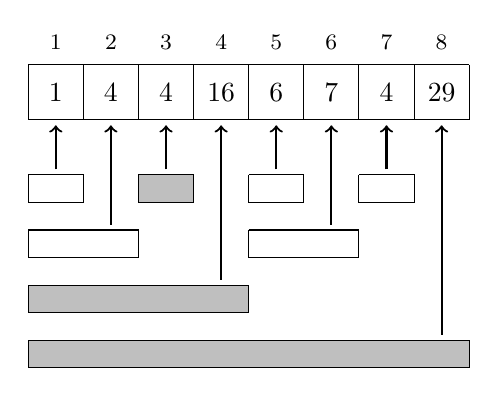
\begin{tikzpicture}[scale=0.7]
\draw (0,0) grid (8,1);

\node at (0.5,0.5) {$1$};
\node at (1.5,0.5) {$4$};
\node at (2.5,0.5) {$4$};
\node at (3.5,0.5) {$16$};
\node at (4.5,0.5) {$6$};
\node at (5.5,0.5) {$7$};
\node at (6.5,0.5) {$4$};
\node at (7.5,0.5) {$29$};

\footnotesize
\node at (0.5,1.4) {$1$};
\node at (1.5,1.4) {$2$};
\node at (2.5,1.4) {$3$};
\node at (3.5,1.4) {$4$};
\node at (4.5,1.4) {$5$};
\node at (5.5,1.4) {$6$};
\node at (6.5,1.4) {$7$};
\node at (7.5,1.4) {$8$};

\draw[->,thick] (0.5,-0.9) -- (0.5,-0.1);
\draw[->,thick] (2.5,-0.9) -- (2.5,-0.1);
\draw[->,thick] (4.5,-0.9) -- (4.5,-0.1);
\draw[->,thick] (6.5,-0.9) -- (6.5,-0.1);
\draw[->,thick] (1.5,-1.9) -- (1.5,-0.1);
\draw[->,thick] (5.5,-1.9) -- (5.5,-0.1);
\draw[->,thick] (3.5,-2.9) -- (3.5,-0.1);
\draw[->,thick] (7.5,-3.9) -- (7.5,-0.1);

\draw (0,-1) -- (1,-1) -- (1,-1.5) -- (0,-1.5) -- (0,-1);
\draw[fill=lightgray] (2,-1) -- (3,-1) -- (3,-1.5) -- (2,-1.5) -- (2,-1);
\draw (4,-1) -- (5,-1) -- (5,-1.5) -- (4,-1.5) -- (4,-1);
\draw (6,-1) -- (7,-1) -- (7,-1.5) -- (6,-1.5) -- (6,-1);
\draw (0,-2) -- (2,-2) -- (2,-2.5) -- (0,-2.5) -- (0,-2);
\draw (4,-2) -- (6,-2) -- (6,-2.5) -- (4,-2.5) -- (4,-2);
\draw[fill=lightgray] (0,-3) -- (4,-3) -- (4,-3.5) -- (0,-3.5) -- (0,-3);
\draw[fill=lightgray] (0,-4) -- (8,-4) -- (8,-4.5) -- (0,-4.5) -- (0,-4);
\end{tikzpicture}
\end{center}

Жиымдағы әр элемент бинарлы индекстелген 
дарақтағы $O(\log n)$ аралығының құрамында
болғандықтан, дарақтағы $O(\log n)$ мәнін өзгерткен
жеткілікті. 

\subsubsection{Кодтың жазылуы}

Бинарлы индекстелген дарақ операцияларын 
биттік операциялар арқылы тиімді жүзеге
асыра аламыз. Бұл жердегі маңызды факт --
әр $p(k)$ мәнін 
\[p(k) = k \& -k.\]
формуласы арқылы есептеу. 

Төмендегі функция $\texttt{sum}_q(1,k)$ мәнін есептейді:
\begin{lstlisting}
int sum(int k) {
    int s = 0;
    while (k >= 1) {
        s += tree[k];
        k -= k&-k;
    }
    return s;
}
\end{lstlisting}

Ал келесі функция жиымның $k$ позициясындағы
мәніне $x$-ті қосады ($x$ оң немесе теріс сан бола алады): 
\begin{lstlisting}
void add(int k, int x) {
    while (k <= n) {
        tree[k] += x;
        k += k&-k;
    }
}
\end{lstlisting}

Екі функцияның уақытша күрделілігі -- $O(\log n)$, 
өйткені функциялар бинарлы индекстелген 
дарақтағы $O(\log n)$ мәнді қарап, әр 
келесі позицияға өту үшін $O(1)$ уақыт жұмсайды. 

\section{Кесінділер дарағы}

\index{кесінділер дарағы}

\key{Кесінділер дарағы}\footnote{Бөлімдегі төменнен жоғарыға қарай код жазылуы \cite{sta06}-ге сәйкес келеді.  Ұқсас құрылымдар 1970 жылдардың аяғында геометриялық есептерді шешу үшін қолданылған \cite{ben80}.} ––
екі түрлі операцияны, атап айтқанда
аралық сұратымдарды өңдеу және жиымдағы мәнді жаңарту операцияларын қолдайтын деректер құрылымы. 
Кесінділер дарағы қосындыны табу, минимум мен максимумды анықтау және басқа да сұратымдарға  $O(\log n)$ уақытта жауап бере алады.

Бинарлы индекстелген дарақпен салыстырғанда кесінділер дарағының артықшылығы -- жалпы деректер құрылымы болуында. Бинарлы индекстелген 
дарақ тек қосынды сұратымдарын қолдаса\footnote{Шын мәнінде
\emph{екі} бинарлы индекстелген дарақ арқылы 
минимум сұратымдарын қолдауға болады \cite{dim15}, бірақ
бұл кесінділер дарағына қарағанда әлдеқайда қиынырақ.}, 
кесінділер дарағы өзге сұратымдарды да қолдайды. 
Есесіне, кесінділер дарағы көп жадыны алады 
және оны кодта жазу сәл қиынырақ болады. 

\subsubsection{Құрылымы}

Кесінділер дарағы -- ең төменгі деңгейде орналасқан төбелері 
жиымның элементтеріне сәйкес келетін және
басқа төбелері аралық сұратымдарды өңдеуге қажет
ақпаратты сақтайтын бинарлы дарақ. 

Бұл бөлімде біз жиымның өлшемі екінің дәрежесіне тең 
және жиым нөлдік индекстелген жағдайды қарастырамыз.
Өйткені мұндай жиым үшін кесінділер дарағын құрастыру
оңайырақ. Егер жиымның өлшемі 
екінің дәрежесі болмаса,
онда біз әрдайым қосымша элементтер қоса аламыз.

Алдымен қосынды аралық сұратымдарын қолдайтын кесінділер
дарағын қарастырайық. Өрнек ретінде төмендегі жиымды алайық:
\begin{center}
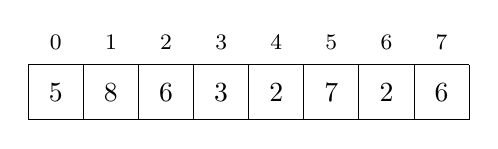
\begin{tikzpicture}[scale=0.7]
\draw (0,0) grid (8,1);

\node at (0.5,0.5) {$5$};
\node at (1.5,0.5) {$8$};
\node at (2.5,0.5) {$6$};
\node at (3.5,0.5) {$3$};
\node at (4.5,0.5) {$2$};
\node at (5.5,0.5) {$7$};
\node at (6.5,0.5) {$2$};
\node at (7.5,0.5) {$6$};

\footnotesize
\node at (0.5,1.4) {$0$};
\node at (1.5,1.4) {$1$};
\node at (2.5,1.4) {$2$};
\node at (3.5,1.4) {$3$};
\node at (4.5,1.4) {$4$};
\node at (5.5,1.4) {$5$};
\node at (6.5,1.4) {$6$};
\node at (7.5,1.4) {$7$};
\end{tikzpicture}
\end{center}
Ол үшін құрылған кесінділер дарағы:
\begin{center}
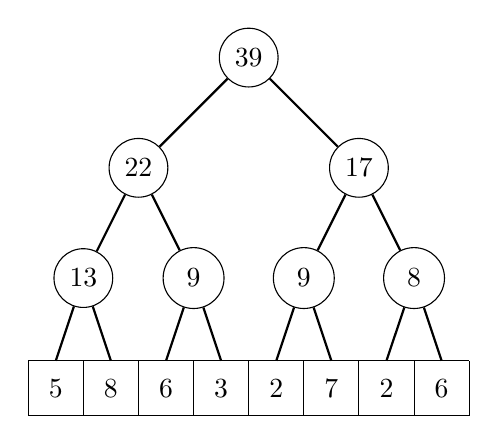
\begin{tikzpicture}[scale=0.7]
\draw (0,0) grid (8,1);

\node[anchor=center] at (0.5, 0.5) {5};
\node[anchor=center] at (1.5, 0.5) {8};
\node[anchor=center] at (2.5, 0.5) {6};
\node[anchor=center] at (3.5, 0.5) {3};
\node[anchor=center] at (4.5, 0.5) {2};
\node[anchor=center] at (5.5, 0.5) {7};
\node[anchor=center] at (6.5, 0.5) {2};
\node[anchor=center] at (7.5, 0.5) {6};

\node[draw, circle] (a) at (1,2.5) {13};
\path[draw,thick,-] (a) -- (0.5,1);
\path[draw,thick,-] (a) -- (1.5,1);
\node[draw, circle,minimum size=22pt] (b) at (3,2.5) {9};
\path[draw,thick,-] (b) -- (2.5,1);
\path[draw,thick,-] (b) -- (3.5,1);
\node[draw, circle,minimum size=22pt] (c) at (5,2.5) {9};
\path[draw,thick,-] (c) -- (4.5,1);
\path[draw,thick,-] (c) -- (5.5,1);
\node[draw, circle,minimum size=22pt] (d) at (7,2.5) {8};
\path[draw,thick,-] (d) -- (6.5,1);
\path[draw,thick,-] (d) -- (7.5,1);

\node[draw, circle] (i) at (2,4.5) {22};
\path[draw,thick,-] (i) -- (a);
\path[draw,thick,-] (i) -- (b);
\node[draw, circle] (j) at (6,4.5) {17};
\path[draw,thick,-] (j) -- (c);
\path[draw,thick,-] (j) -- (d);

\node[draw, circle] (m) at (4,6.5) {39};
\path[draw,thick,-] (m) -- (i);
\path[draw,thick,-] (m) -- (j);
\end{tikzpicture}
\end{center}

Дарақтағы әрбір ішкі төбенің 
өлшемі -- екінің дәрежесі болатын жиымға
пара-пар. Келтірілген дарақтағы ішкі 
төбелердің мәні -- сәйкес келетін 
жиым элементтерінің қосындысы.
Олар сол және оң жақтағы
ұл төбелердің қосындысына тең болады.

$[a,b]$ аралығының кез келген 
мәндері дарақтағы төбелерде сақталған
$O(\log n)$ аралықтарға бөлінеді екен.
Мысалы, [2,7] аралығын қарастырайық:
\begin{center}
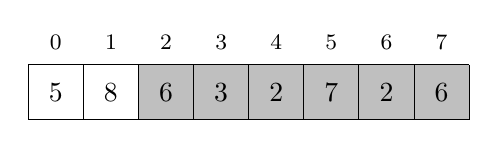
\begin{tikzpicture}[scale=0.7]
\fill[color=gray!50] (2,0) rectangle (8,1);
\draw (0,0) grid (8,1);

\node[anchor=center] at (0.5, 0.5) {5};
\node[anchor=center] at (1.5, 0.5) {8};
\node[anchor=center] at (2.5, 0.5) {6};
\node[anchor=center] at (3.5, 0.5) {3};
\node[anchor=center] at (4.5, 0.5) {2};
\node[anchor=center] at (5.5, 0.5) {7};
\node[anchor=center] at (6.5, 0.5) {2};
\node[anchor=center] at (7.5, 0.5) {6};

\footnotesize
\node at (0.5,1.4) {$0$};
\node at (1.5,1.4) {$1$};
\node at (2.5,1.4) {$2$};
\node at (3.5,1.4) {$3$};
\node at (4.5,1.4) {$4$};
\node at (5.5,1.4) {$5$};
\node at (6.5,1.4) {$6$};
\node at (7.5,1.4) {$7$};
\end{tikzpicture}
\end{center}
Бұл жерде $\texttt{sum}_q(2,7)=6+3+2+7+2+6=26$.
Біздің жағдайда төменде берілген
дарақтағы екі төбе аралыққа сәйкес
келеді:
\begin{center}
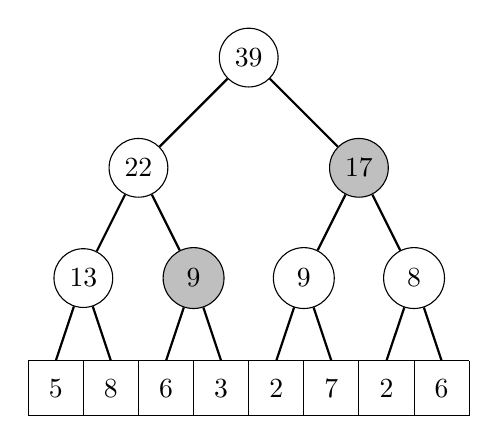
\begin{tikzpicture}[scale=0.7]
\draw (0,0) grid (8,1);

\node[anchor=center] at (0.5, 0.5) {5};
\node[anchor=center] at (1.5, 0.5) {8};
\node[anchor=center] at (2.5, 0.5) {6};
\node[anchor=center] at (3.5, 0.5) {3};
\node[anchor=center] at (4.5, 0.5) {2};
\node[anchor=center] at (5.5, 0.5) {7};
\node[anchor=center] at (6.5, 0.5) {2};
\node[anchor=center] at (7.5, 0.5) {6};

\node[draw, circle] (a) at (1,2.5) {13};
\path[draw,thick,-] (a) -- (0.5,1);
\path[draw,thick,-] (a) -- (1.5,1);
\node[draw, circle,fill=gray!50,minimum size=22pt] (b) at (3,2.5) {9};
\path[draw,thick,-] (b) -- (2.5,1);
\path[draw,thick,-] (b) -- (3.5,1);
\node[draw, circle,minimum size=22pt] (c) at (5,2.5) {9};
\path[draw,thick,-] (c) -- (4.5,1);
\path[draw,thick,-] (c) -- (5.5,1);
\node[draw, circle,minimum size=22pt] (d) at (7,2.5) {8};
\path[draw,thick,-] (d) -- (6.5,1);
\path[draw,thick,-] (d) -- (7.5,1);

\node[draw, circle] (i) at (2,4.5) {22};
\path[draw,thick,-] (i) -- (a);
\path[draw,thick,-] (i) -- (b);
\node[draw, circle,fill=gray!50] (j) at (6,4.5) {17};
\path[draw,thick,-] (j) -- (c);
\path[draw,thick,-] (j) -- (d);

\node[draw, circle] (m) at (4,6.5) {39};
\path[draw,thick,-] (m) -- (i);
\path[draw,thick,-] (m) -- (j);
\end{tikzpicture}
\end{center}
Осылайша, қосындыны есептеудің тағы бір жолы -- $9+17=26$ болып шығады.

Қосындыны мүмкіндігінше ең жоғарғы төбелер
арқылы есептейтін болсақ, дарақтағы 
әр деңгейде ең көбі екі төбе қажет болады. Демек
жалпы төбелер саны -- $O(\log n)$.

Жиымды жаңартқаннан кейін 
өзгерген мәнге тәуелді 
барлық төбелерді жаңартуымыз қажет.
Мұны өзгерген жиым элементінен бастап
ең жоғарғы төбеге дейінгі жолмен жүріп, 
жолдағы төбелерді өзгерту арқылы жүзеге асырамыз. 

Төмендегі сурет 7 мәні өзгерсе, дарақтағы 
қандай төбелер өзгеретінін көрсетеді:

\begin{center}
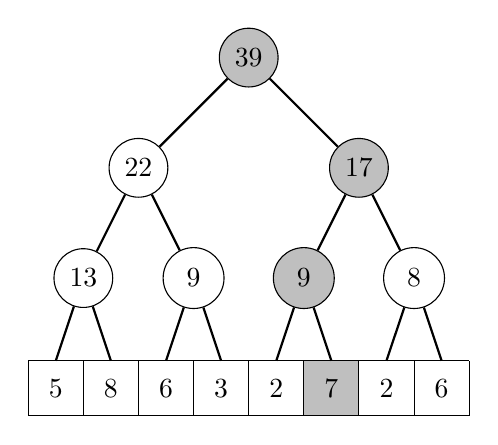
\begin{tikzpicture}[scale=0.7]
\fill[color=gray!50] (5,0) rectangle (6,1);
\draw (0,0) grid (8,1);

\node[anchor=center] at (0.5, 0.5) {5};
\node[anchor=center] at (1.5, 0.5) {8};
\node[anchor=center] at (2.5, 0.5) {6};
\node[anchor=center] at (3.5, 0.5) {3};
\node[anchor=center] at (4.5, 0.5) {2};
\node[anchor=center] at (5.5, 0.5) {7};
\node[anchor=center] at (6.5, 0.5) {2};
\node[anchor=center] at (7.5, 0.5) {6};

\node[draw, circle] (a) at (1,2.5) {13};
\path[draw,thick,-] (a) -- (0.5,1);
\path[draw,thick,-] (a) -- (1.5,1);
\node[draw, circle,minimum size=22pt] (b) at (3,2.5) {9};
\path[draw,thick,-] (b) -- (2.5,1);
\path[draw,thick,-] (b) -- (3.5,1);
\node[draw, circle,minimum size=22pt,fill=gray!50] (c) at (5,2.5) {9};
\path[draw,thick,-] (c) -- (4.5,1);
\path[draw,thick,-] (c) -- (5.5,1);
\node[draw, circle,minimum size=22pt] (d) at (7,2.5) {8};
\path[draw,thick,-] (d) -- (6.5,1);
\path[draw,thick,-] (d) -- (7.5,1);

\node[draw, circle] (i) at (2,4.5) {22};
\path[draw,thick,-] (i) -- (a);
\path[draw,thick,-] (i) -- (b);
\node[draw, circle,fill=gray!50] (j) at (6,4.5) {17};
\path[draw,thick,-] (j) -- (c);
\path[draw,thick,-] (j) -- (d);

\node[draw, circle,fill=gray!50] (m) at (4,6.5) {39};
\path[draw,thick,-] (m) -- (i);
\path[draw,thick,-] (m) -- (j);
\end{tikzpicture}
\end{center}

Төменнен жоғарыға дейінгі жол
әрдайым $O(\log n)$ төбеден тұрады, 
сондықтан әр жаңарту дарақтағы 
$O(\log n)$ төбені жаңартады. 

\subsubsection{Кодтың жазылуы}

Біз кесінділер дарағын $2n$ элементтен 
тұратын жиымда сақтайтын боламыз, 
мұндағы $n$ берілген жиымның өлшемі және ол
екінің дәрежесіне тең. Дарақтың төбелері 
жоғарыдан төменге қарай сақталады. Мұндағы
$\texttt{tree}[1]$ --ң жоғарғы төбе, 
$\texttt{tree}[2]$ және $\texttt{tree}[3]$ --
оның ұлдары болып жалғаса береді. Соңында $\texttt{tree}[n]$ 
мен $\texttt{tree}[2n-1]$ аралығында орналасқан
дарақтың төменгі деңгейіндегі мәндер --
берілген жиым мәндеріне сәйкес келеді.

Мысалы, төмендегі кесінділер дарағы
\begin{center}
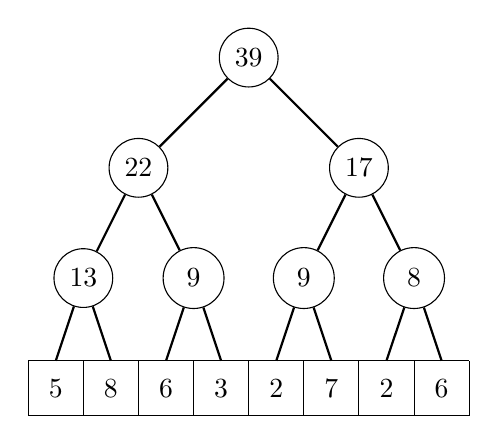
\begin{tikzpicture}[scale=0.7]
\draw (0,0) grid (8,1);

\node[anchor=center] at (0.5, 0.5) {5};
\node[anchor=center] at (1.5, 0.5) {8};
\node[anchor=center] at (2.5, 0.5) {6};
\node[anchor=center] at (3.5, 0.5) {3};
\node[anchor=center] at (4.5, 0.5) {2};
\node[anchor=center] at (5.5, 0.5) {7};
\node[anchor=center] at (6.5, 0.5) {2};
\node[anchor=center] at (7.5, 0.5) {6};

\node[draw, circle] (a) at (1,2.5) {13};
\path[draw,thick,-] (a) -- (0.5,1);
\path[draw,thick,-] (a) -- (1.5,1);
\node[draw, circle,minimum size=22pt] (b) at (3,2.5) {9};
\path[draw,thick,-] (b) -- (2.5,1);
\path[draw,thick,-] (b) -- (3.5,1);
\node[draw, circle,minimum size=22pt] (c) at (5,2.5) {9};
\path[draw,thick,-] (c) -- (4.5,1);
\path[draw,thick,-] (c) -- (5.5,1);
\node[draw, circle,minimum size=22pt] (d) at (7,2.5) {8};
\path[draw,thick,-] (d) -- (6.5,1);
\path[draw,thick,-] (d) -- (7.5,1);

\node[draw, circle] (i) at (2,4.5) {22};
\path[draw,thick,-] (i) -- (a);
\path[draw,thick,-] (i) -- (b);
\node[draw, circle] (j) at (6,4.5) {17};
\path[draw,thick,-] (j) -- (c);
\path[draw,thick,-] (j) -- (d);

\node[draw, circle] (m) at (4,6.5) {39};
\path[draw,thick,-] (m) -- (i);
\path[draw,thick,-] (m) -- (j);
\end{tikzpicture}
\end{center}
төмендегі үлгіде сақталады:
\begin{center}
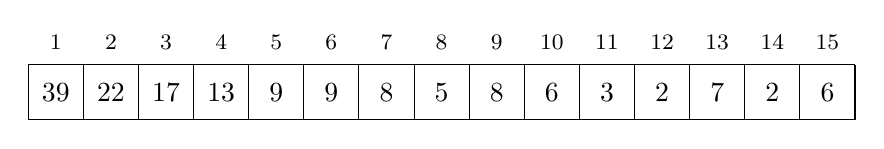
\begin{tikzpicture}[scale=0.7]
\draw (0,0) grid (15,1);

\node at (0.5,0.5) {$39$};
\node at (1.5,0.5) {$22$};
\node at (2.5,0.5) {$17$};
\node at (3.5,0.5) {$13$};
\node at (4.5,0.5) {$9$};
\node at (5.5,0.5) {$9$};
\node at (6.5,0.5) {$8$};
\node at (7.5,0.5) {$5$};
\node at (8.5,0.5) {$8$};
\node at (9.5,0.5) {$6$};
\node at (10.5,0.5) {$3$};
\node at (11.5,0.5) {$2$};
\node at (12.5,0.5) {$7$};
\node at (13.5,0.5) {$2$};
\node at (14.5,0.5) {$6$};

\footnotesize
\node at (0.5,1.4) {$1$};
\node at (1.5,1.4) {$2$};
\node at (2.5,1.4) {$3$};
\node at (3.5,1.4) {$4$};
\node at (4.5,1.4) {$5$};
\node at (5.5,1.4) {$6$};
\node at (6.5,1.4) {$7$};
\node at (7.5,1.4) {$8$};
\node at (8.5,1.4) {$9$};
\node at (9.5,1.4) {$10$};
\node at (10.5,1.4) {$11$};
\node at (11.5,1.4) {$12$};
\node at (12.5,1.4) {$13$};
\node at (13.5,1.4) {$14$};
\node at (14.5,1.4) {$15$};
\end{tikzpicture}
\end{center}
Осы көріністі қолдана отырып,
$\texttt{tree}[k]$-ның әкесі 
$\texttt{tree}[\lfloor k/2 \rfloor]$ болады,
ал ұлдарына $\texttt{tree}[2k]$
мен $\texttt{tree}[2k+1]$ жатады.
Осылайша, төбенің позициясы жұп болса, онда ол сол жақ ұлы,
ал тақ болса, ол оң жақ ұлы екенін көрсетеді. 

Төмендегі функция $\texttt{sum}_q(a,b)$
мәнін есептейді:
\begin{lstlisting}
int sum(int a, int b) {
    a += n; b += n;
    int s = 0;
    while (a <= b) {
        if (a%2 == 1) s += tree[a++];
        if (b%2 == 0) s += tree[b--];
        a /= 2; b /= 2;
    }
    return s;
}
\end{lstlisting}
Функция басында $[a+n,b+n]$ аралықты
ұстап тұрады. Сосын келесі қадамда
аралық бір деңгей жоғары қозғалады 
және оған дейін үстіңгі аралыққа 
кірмейтін төбелердің мәні қосындыға қосылады.

Төмендегі функция $k$ позициясындағы жиым мәнін 
$x$-ке арттырады:
\begin{lstlisting}
void add(int k, int x) {
    k += n;
    tree[k] += x;
    for (k /= 2; k >= 1; k /= 2) {
        tree[k] = tree[2*k]+tree[2*k+1];
    }
}
\end{lstlisting}
Алдымен функция дарақтың төменгі 
деңгейіндегі мәнді жаңартады.
Кейін дарақтың жоғарғы 
төбесіне жеткенге дейін, барлық ішкі 
төбелердің мәндерін жаңартады.

Үстідегі екі фукнция $O(\log n)$ уақытта
жұмыс істейді: $n$ элементтен тұратын
кесінділер дарағы $O(\log n)$ деңгейден
тұрады және әр қадам сайын 
бір деңгей жоғары көтеріледі. 

\subsubsection{Басқа сұратымдар}

Кесінділер дарағы аралықты екіге бөліп,
жауапты бөлек есептеп, кейін оларды тиімді 
біріктіретін барлық аралық сұратымдарды қолдайды. 
Осы типтегі сұратымдар -- минимум, максимум, ең үлкен 
ортақ бөлгіш және биттік операциялар -- конъюнкция, дизъюнкция, жоюшы дизъюнкция (xor). % TODO.

Мысалы, төмендегі кесінділер дарағы минимум
сұратымдарды қолдайды:

\begin{center}
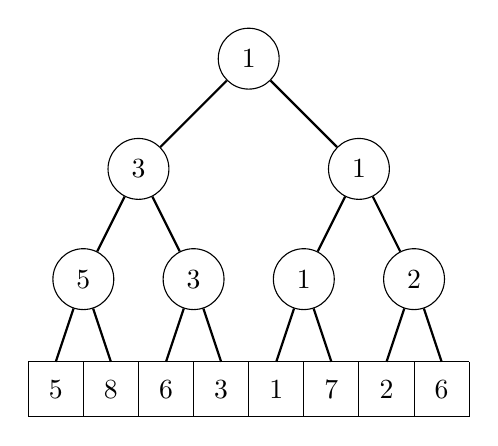
\begin{tikzpicture}[scale=0.7]
\draw (0,0) grid (8,1);

\node[anchor=center] at (0.5, 0.5) {5};
\node[anchor=center] at (1.5, 0.5) {8};
\node[anchor=center] at (2.5, 0.5) {6};
\node[anchor=center] at (3.5, 0.5) {3};
\node[anchor=center] at (4.5, 0.5) {1};
\node[anchor=center] at (5.5, 0.5) {7};
\node[anchor=center] at (6.5, 0.5) {2};
\node[anchor=center] at (7.5, 0.5) {6};

\node[draw, circle,minimum size=22pt] (a) at (1,2.5) {5};
\path[draw,thick,-] (a) -- (0.5,1);
\path[draw,thick,-] (a) -- (1.5,1);
\node[draw, circle,minimum size=22pt] (b) at (3,2.5) {3};
\path[draw,thick,-] (b) -- (2.5,1);
\path[draw,thick,-] (b) -- (3.5,1);
\node[draw, circle,minimum size=22pt] (c) at (5,2.5) {1};
\path[draw,thick,-] (c) -- (4.5,1);
\path[draw,thick,-] (c) -- (5.5,1);
\node[draw, circle,minimum size=22pt] (d) at (7,2.5) {2};
\path[draw,thick,-] (d) -- (6.5,1);
\path[draw,thick,-] (d) -- (7.5,1);

\node[draw, circle,minimum size=22pt] (i) at (2,4.5) {3};
\path[draw,thick,-] (i) -- (a);
\path[draw,thick,-] (i) -- (b);
\node[draw, circle,minimum size=22pt] (j) at (6,4.5) {1};
\path[draw,thick,-] (j) -- (c);
\path[draw,thick,-] (j) -- (d);

\node[draw, circle,minimum size=22pt] (m) at (4,6.5) {1};
\path[draw,thick,-] (m) -- (i);
\path[draw,thick,-] (m) -- (j);
\end{tikzpicture}
\end{center}

Бұл жағдайда дарақтың әр төбесі 
жиымның аралығына сәйкес ең кіші мәнді сақтайды.
Дарақтағы ең жоғарғы төбе бүкіл жиымның ең кішкентай мәнін
сақтайды. Операцияларды бұрынғыдай орындауға болады, бірақ бұл жағдайда
қосындылар орнына минимумдар есептеледі.

Кесінділер дарағының құрылымы жиымның элементтерін 
бинарлық ізденіс арқылы табуға
жол береді. Мысалы, егер дарақ минимум сұратымдарын
қолдаса, онда ең кішкентай элементтің позициясын 
$O(\log n)$ уақытта таба аламыз. 

Мысалы, келтірілген дарақта ең кіші мәні 1 болатын 
элементті жоғарыдан төменге қарай жүру арқылы табуға болады:

\begin{center}
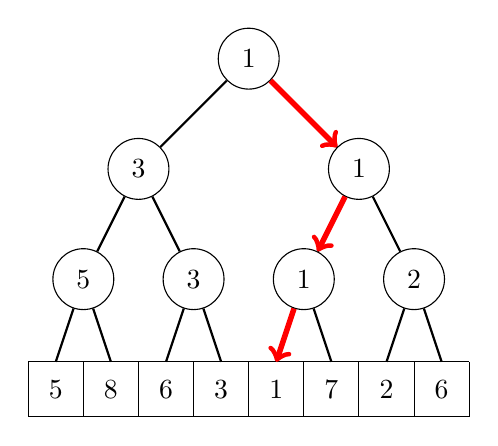
\begin{tikzpicture}[scale=0.7]
\draw (0,0) grid (8,1);

\node[anchor=center] at (0.5, 0.5) {5};
\node[anchor=center] at (1.5, 0.5) {8};
\node[anchor=center] at (2.5, 0.5) {6};
\node[anchor=center] at (3.5, 0.5) {3};
\node[anchor=center] at (4.5, 0.5) {1};
\node[anchor=center] at (5.5, 0.5) {7};
\node[anchor=center] at (6.5, 0.5) {2};
\node[anchor=center] at (7.5, 0.5) {6};

\node[draw, circle,minimum size=22pt] (a) at (1,2.5) {5};
\path[draw,thick,-] (a) -- (0.5,1);
\path[draw,thick,-] (a) -- (1.5,1);
\node[draw, circle,minimum size=22pt] (b) at (3,2.5) {3};
\path[draw,thick,-] (b) -- (2.5,1);
\path[draw,thick,-] (b) -- (3.5,1);
\node[draw, circle,minimum size=22pt] (c) at (5,2.5) {1};
\path[draw,thick,-] (c) -- (4.5,1);
\path[draw,thick,-] (c) -- (5.5,1);
\node[draw, circle,minimum size=22pt] (d) at (7,2.5) {2};
\path[draw,thick,-] (d) -- (6.5,1);
\path[draw,thick,-] (d) -- (7.5,1);

\node[draw, circle,minimum size=22pt] (i) at (2,4.5) {3};
\path[draw,thick,-] (i) -- (a);
\path[draw,thick,-] (i) -- (b);
\node[draw, circle,minimum size=22pt] (j) at (6,4.5) {1};
\path[draw,thick,-] (j) -- (c);
\path[draw,thick,-] (j) -- (d);

\node[draw, circle,minimum size=22pt] (m) at (4,6.5) {1};
\path[draw,thick,-] (m) -- (i);
\path[draw,thick,-] (m) -- (j);

\path[draw=red,thick,->,line width=2pt] (m) -- (j);
\path[draw=red,thick,->,line width=2pt] (j) -- (c);
\path[draw=red,thick,->,line width=2pt] (c) -- (4.5,1);
\end{tikzpicture}
\end{center}

\section{Қосымша әдіс-тәсілдер}

\subsubsection{Индекстерді сығымдау}
% TODO
Жиымнан құрылған  деректер құрылымының 
шектеуі элементтердің қатар орналасқан 
сандар арқылы индекстелуімен байланыстырылады.
Үлкен индекстер 
қажет болған жағдайда қиындық туындайды. 
Мысалы, егер $10^9$ индексін қолданғымыз
келсе, сәйкесінше, жиым $10^9$ элементтен тұруы шарт.
Ол өз кезегінде тым көп жадыны талап етеді. 

\index{индекстерді сығымдау}

Алайда туындаған қиындықты сығымдау
арқылы шешуге болады, яғни бастапқы индекстерді
1, 2, 3 сияқты индекстерге алмастырамыз.
Мұны алгоритмге қажет барлық индекстерді
алдын ала білген жағдайда ғана іске асыра аламыз.

Идеясы әр түпкі $x$ индексін $c(x)$-пен ауыстыруға негізделген. 
Мұндағы $c$ -- индекстерді сығымдайтын функция. Бұл жерде 
индекстер ретінің өзгермеуін талап еткеніміз жөн, 
яғни $a<b$ болса, $c(a)<c(b)$ болуы керек.
Бұл индекстер сығымдалған болса да сұратымдарды
ыңғайлы орындауға мүмкіндік береді. 

Мысалы, түпкі индекстер $555$, $10^9$ және 
$8$ болса, жаңа индекстер төмендегідей болады:

\[
\begin{array}{lcl}
c(8) & = & 1 \\
c(555) & = & 2 \\
c(10^9) & = & 3 \\
\end{array}
\]

\subsubsection{Аралық жаңартулар}

Осыған дейін біз аралық сұратымдарды 
қолдайтын және бір ғана мәнді өзгертетін
деректер құрылымының кодын жаздық. 
Енді теріс жағдайды, яғни
аралықты жаңартатын және бір ғана мәнді 
қарайтын сұратымдарды, $[a,b]$ аралығындағы
барлық элементтерді
$x$–ке арттыратын операцияны ғана қарастырайық.

\index{айырма жиымы}

Бөлімде аталған деректер құрылымын 
осы жағдайда да қолдануға болады. 
Ол үшін берілген жиымдағы
қатар мәндер арасындағы айырмашылықтарды 
көрсететін \key{айырма жиымын} құрастырамыз.
Осылайша, берілген жиым -- айырма жиымның префиксті
қосындылар жиымы болады. 
Мысалы, келесі жиымды қарастырайық:

\begin{center}
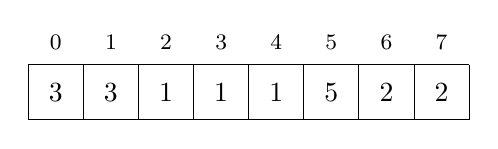
\begin{tikzpicture}[scale=0.7]
\draw (0,0) grid (8,1);

\node at (0.5,0.5) {$3$};
\node at (1.5,0.5) {$3$};
\node at (2.5,0.5) {$1$};
\node at (3.5,0.5) {$1$};
\node at (4.5,0.5) {$1$};
\node at (5.5,0.5) {$5$};
\node at (6.5,0.5) {$2$};
\node at (7.5,0.5) {$2$};


\footnotesize
\node at (0.5,1.4) {$0$};
\node at (1.5,1.4) {$1$};
\node at (2.5,1.4) {$2$};
\node at (3.5,1.4) {$3$};
\node at (4.5,1.4) {$4$};
\node at (5.5,1.4) {$5$};
\node at (6.5,1.4) {$6$};
\node at (7.5,1.4) {$7$};
\end{tikzpicture}
\end{center}

Айырма жиымы төмендегідей болады:
\begin{center}
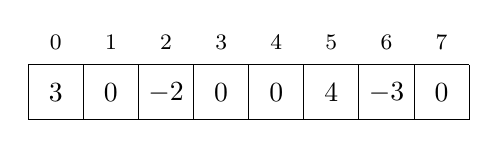
\begin{tikzpicture}[scale=0.7]
\draw (0,0) grid (8,1);

\node at (0.5,0.5) {$3$};
\node at (1.5,0.5) {$0$};
\node at (2.5,0.5) {$-2$};
\node at (3.5,0.5) {$0$};
\node at (4.5,0.5) {$0$};
\node at (5.5,0.5) {$4$};
\node at (6.5,0.5) {$-3$};
\node at (7.5,0.5) {$0$};


\footnotesize
\node at (0.5,1.4) {$0$};
\node at (1.5,1.4) {$1$};
\node at (2.5,1.4) {$2$};
\node at (3.5,1.4) {$3$};
\node at (4.5,1.4) {$4$};
\node at (5.5,1.4) {$5$};
\node at (6.5,1.4) {$6$};
\node at (7.5,1.4) {$7$};
\end{tikzpicture}
\end{center}

Берілген жиымдағы 6-позициядағы 2 мәні 
айырма жиымындағы $3-2+4-3=2$ қосындысына сәйкес келеді. 

Айырма жиымының артықшылығы -- берілген жиымдағы 
аралықты жаңарту үшін өзінің екі ғана
элементін өзгеруінде. Мысалы, берілген жиымдағы 
1 және 4-позиция аралығын 5-ке арттыру үшін 
айырма жиымында 1-позициядағы санды 5-ке арттырып,
5-позициядағы санды 5-ке азайту жеткілікті. 
Нәтижесінде :

\begin{center}
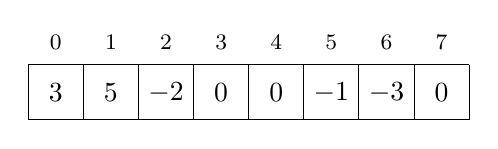
\begin{tikzpicture}[scale=0.7]
\draw (0,0) grid (8,1);

\node at (0.5,0.5) {$3$};
\node at (1.5,0.5) {$5$};
\node at (2.5,0.5) {$-2$};
\node at (3.5,0.5) {$0$};
\node at (4.5,0.5) {$0$};
\node at (5.5,0.5) {$-1$};
\node at (6.5,0.5) {$-3$};
\node at (7.5,0.5) {$0$};

\footnotesize
\node at (0.5,1.4) {$0$};
\node at (1.5,1.4) {$1$};
\node at (2.5,1.4) {$2$};
\node at (3.5,1.4) {$3$};
\node at (4.5,1.4) {$4$};
\node at (5.5,1.4) {$5$};
\node at (6.5,1.4) {$6$};
\node at (7.5,1.4) {$7$};
\end{tikzpicture}
\end{center}

Қорыта айтқанда $[a,b]$ аралығын $x$-ке
арттыру үшін біз $a$ позициясындағы санды $x$-ке
арттырып, $b+1$ позициядағы санды $x$-ке азайтамыз.
Демек тек бір мәнді жаңарту және қосынды сұратымдарын
өңдеу қажет. Ал ол үшін біз бинарлы индекстелген дарақ
немесе кесінділер дарағын қолдана аламыз.

Сәл қиынырақ есепке
аралық сұратымдарды және аралық жаңартуларды қолдау жатады.
28-тарауда біз мұның мүмкін екенін көреміз.


